\documentclass{article}

\usepackage{url} 

\usepackage{pdfpages}
\usepackage{lastpage}
\usepackage{fancyhdr}
\usepackage{ngerman}
\usepackage{listings}

\usepackage{floatrow}
\usepackage[tableposition=top]{caption}
\floatsetup[table]{capposition=top}

\usepackage{amsmath, amssymb}

\usepackage[utf8]{inputenc}


\usepackage[numbib]{tocbibind}



\newcommand\twodigits[1]{%
   \ifnum#1<10 0#1\else #1\fi
}



\lhead{Halbschattenpolarimeter}
\rhead{16. Oktober 2020\\T. Maier, J. Winkler}
%\cfoot{\twodigits{\thepage}~/ \pageref{LastPage}}
\cfoot{{\thepage}~/ \pageref{LastPage}}

\newcommand{\as}{\alpha_\text{spez}}

\begin{document}

\parindent0cm

%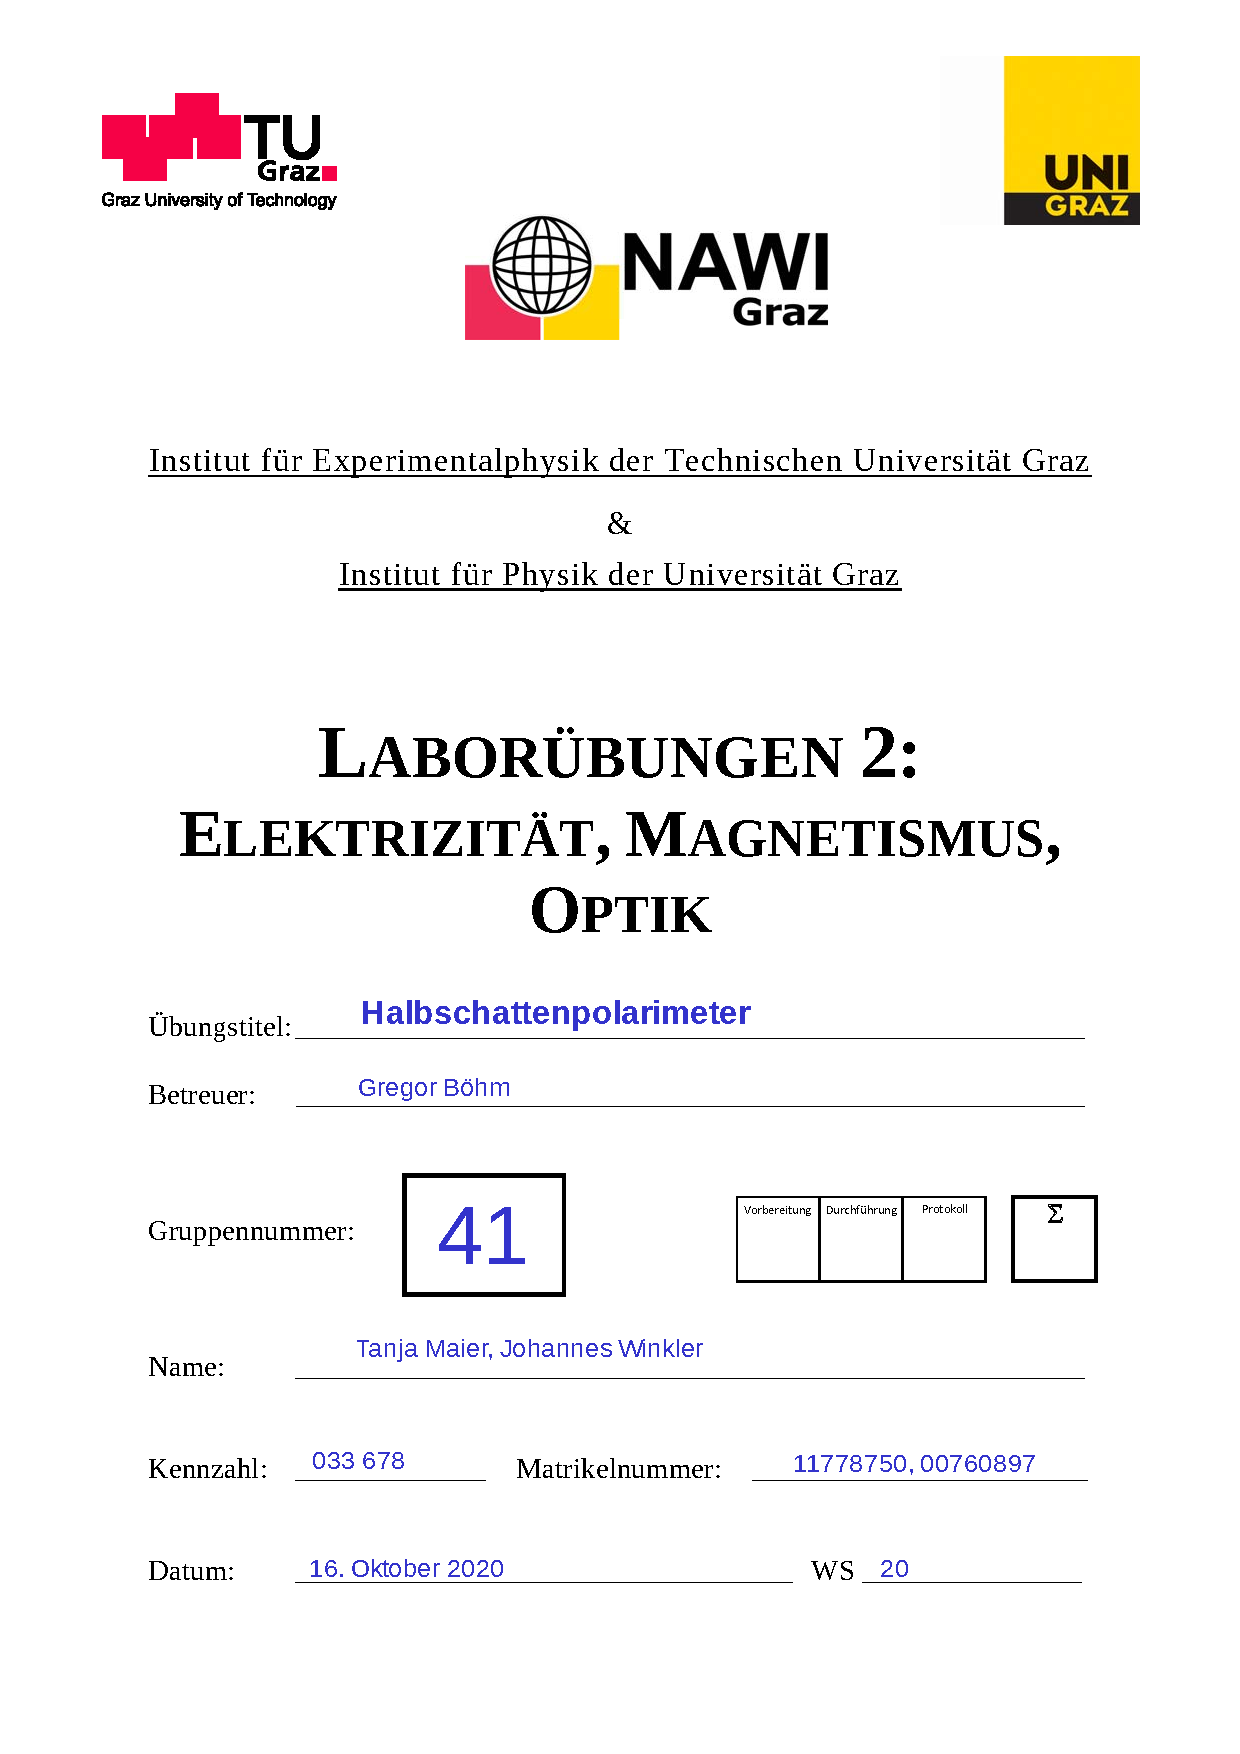
\includepdf{Deckblatt.pdf}


\pagestyle{fancy}

\section{Aufgabenstellung}

\begin{enumerate}
\item Bestimmung der Konzentration einer Rohrzuckerlösung.
\item Bestimmung der spezifischen Drehung einer Quarzplatte.
\end{enumerate}

\section{Grundlagen und Versuchsaufbau}

Unter optischer Aktivität versteht man die Eigenschaft mancher Medien, die Schwingungsebene linear polarisierten Lichts nach rechts oder links zu drehen. Dieses Verhalten wird durch eine schraubenfömige Struktur des Kristallgitters (bei festen Stoffen) bzw. der Moleküle (bei Flüssigkeiten und Gasen) hervorgerufen. Denkt man sich die linear polarisierte Welle aus zweientgegengesetzt zirkular polarisierten Wellen zusammengesetzt, können die beiden Anteile in einem solchen Medium unterschiedliche Ausbreitungsgeschwindigkeiten besitzen. Sie treten daher aus dem Medium mit einer Phasendifferenz aus, und setzen sich zu einer linear polarisierten Welle mit gedrehter Polarisationsrichtung zusammen. Die Größe des Winkels $\alpha$ ist von der durchlaufenen Wegstrecke $d$ bzw. $\ell$, der spezifischen Drehung $\as$ und der Konzentration des Mediums $c$ abhängig.

\begin{equation}
\label{eq:main}
\begin{aligned}
  \alpha &= \as\cdot \ell \cdot c && \text{für Flüssigkeiten und Gase} \\
  \alpha &= \as\cdot d && \text{für Kristalle und Festkörper}
\end{aligned}
\end{equation}

Um aus natürlichem Licht linear polarisiertes zu erhalten, kann z.B. ein Nicol'sches Prismaverwendet werden. Es besteht aus einem geeignet ausgerichteten und geschnittenen doppelbrechenden Kristall. Dabei wird eintretendes unpolarisiertes Licht in zwei senkrecht zueinanderstehende linear polarisierte Anteile mit unterschiedlicher Ausbreitungsgeschwindigkeit aufgespalten. Durch Totalreflexion eines der beiden Anteile an einer Grenzfläche können die beiden Polarisationsanteile voneinander getrennt werden.

Da es aus physiologischen Gründen schwierig ist, eine Polarisator – Analysator – Anordnung aufmaximale oder minimale Helligkeit abzugleichen, wird für Messzwecke ein sog. Halbschattenpolarimeter (Abb. \ref{fig:halbschattenpolarimeter}) verwendet. Dabei wird nach dem Polarisator ein nur den halben Strahlengangbedeckendes zweites Nicol'sches Prisma eingesetzt, das um einen kleinen Winkel gegen den Pola-risator verdreht ist. Beim Durchstimmen des Analysators beobachtet man in dem nun geteiltenGesichtsfeld nacheinander ein Helligkeitsminimum in beiden Hälften. Befindet sich der Analysator genau senkrecht zum Symmetriewinkel zwischen Polarisator und Halbschattenprisma,erscheinen beide Gesichtsfeldhälften gleich hell. Die Trennlinie ist nicht sichtbar. Bei einer ge-ringen Abweichung von dieser Stellung wird eine der beiden Hälften sofort dunkler. Dadurch istein präziser Abgleich der Polarisator – Analysatorstellung möglich.


\begin{figure}[H]
\centering
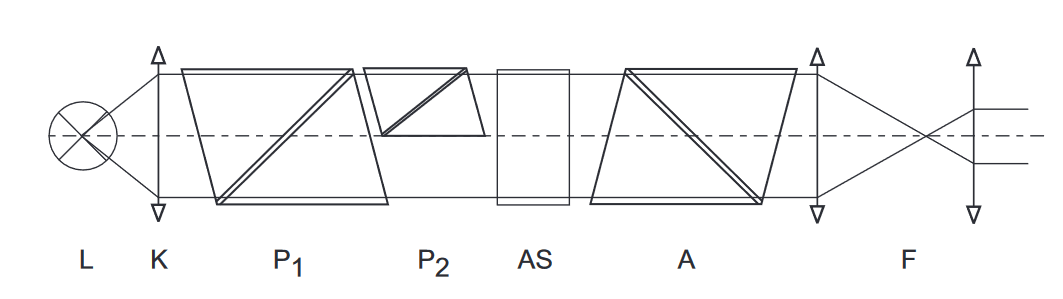
\includegraphics[scale=0.4]{halbschattenpolarimeter.png}
\caption{Aufbau des Halbschattenpolarimeters $L$ Na-Dampflampe, $K$ Kondensor, $P_1$ Polarisator, $P_2$ Halbschattenprisma, $AS$ optisch aktive Substanz, $A$ Analysator, $F$ Fernrohr}
\label{fig:halbschattenpolarimeter}
\end{figure}

\newpage

\section{Geräteliste}

\begin{table}[H]
\caption{Liste der verwendeten Geräte}

~

\begin{tabular}{l|llll}
Bezeichnung & Gerätenummer & Unsicherheit \\
\hline
Micrometer & & $\pm~0.01~$mm \\
1. Halbschattenpolarimeter & & $\pm~0.05~^\circ$ \\
2. Halbschattenpolarimeter & & $\pm~0.1~^\circ$ \\
Schiebelehre & & $\pm~0.05~$mm \\
Rohrzuckerlösung & & \\
Quarzkristalle & & 
\end{tabular}

\end{table}




\section{Durchführung und Messwerte}

\subsection{Rohrzuckerlösung}

\begin{table}[H]
\caption{Rohrzuckerlösung in Probenglas, Abmessungen. $\ell_\text{ges}$ Gesamtlänge, $\ell_1$ innere Länge 1, $\ell_2$ innere Länge 2.}
\label{tab:rohrzucker_abmessungen}
\centering
\begin{tabular}{rrr}\\
 $\ell_\text{ges}$ / mm & $\ell_1$ / mm & $\ell_2$ /mm \\
 \hline
111.70 & 3.85 & 3.85\\
111.65 & 3.80 & 3.85\\
111.70 & 3.85 & 3.80\\
111.70 & 3.85 & 3.85\\
111.60 & 3.85 & 3.85
\end{tabular}
\end{table}




\begin{table}[H]
\caption{Offset und Drehwinkel der Rohrzuckerlösung.}
\label{tab:rohrzucker_winkel}
\centering
\begin{tabular}{r|r}\\
 $\alpha_\text{off}$ / ${}^\circ$ & $\alpha_1$ / ${}^\circ$  \\
 \hline
0.00 & 4.40\\
0.00 & 4.40\\
0.00 & 4.50\\
0.00 & 4.60\\
0.00 & 4.70\\
0.00 & 4.40\\
0.00 & 4.40\\
0.00 & 4.45\\
0.00 & 4.50\\
0.00 & 4.35
\end{tabular}
\end{table}


\subsection{Quarzkristalle}


\begin{table}[H]
\caption{Dicken der Quarzkristalle.}
\label{tab:kristalle_dicken}
\centering
\begin{tabular}{rrrr}\\
 $d_1$ / mm & $d_2$ / mm & $d_3$ / mm & $d_4$ / mm  \\
 \hline
6.99 & 6.51 & 9.17 & 9.43\\
6.98 & 6.50 & 9.16 & 9.43\\
6.99 & 6.50 & 9.17 & 9.42\\
6.98 & 6.51 & 9.16 & 9.43\\
6.99 & 6.51 & 9.16 & 9.42
\end{tabular}
\end{table}




\begin{table}[H]
\caption{Offset und Drehwinkel der Quarzkristalle.}
\label{tab:kristall_winkel}
\centering
\begin{tabular}{r|rrrr}\\
 $\alpha_\text{off}$ / ${}^\circ$ & $\alpha_1$ / ${}^\circ$ & $\alpha_2$ / ${}^\circ$ & $\alpha_3$ / ${}^\circ$ & $\alpha_4$ / ${}^\circ$  \\
 \hline
14.90 & 43.80 & 53.80 & -5.10 & 40.70\\
15.00 & 43.90 & 53.60 & -5.00 & 40.80\\
15.10 & 43.70 & 53.70 & -4.90 & 40.60\\
15.00 & 43.80 & 53.50 & -5.00 & 40.80\\
15.10 & 43.70 & 53.50 & -4.90 & 40.70
\end{tabular}
\end{table}


\section{Auswertung}


\subsection{Rohrzuckerlösung}
Zuerst wird die Länge des Probenglases bestimmt werden, in dem sich die Flüssigkeit befindet.
\begin{align*}
\ell = \ell_\text{ges} - \ell_1 - \ell_2
\end{align*}
Mit Fehlerrechnung ergibt sich
\begin{align*}\\
\ell = (103.99 \pm0.03)~\text{mm} \\
\end{align*}\\


Bestimmung der Konzentration mit Gleichung \eqref{eq:main}
\begin{align*}
c &= \frac{\alpha}{\as\cdot \ell} \\
\Delta c &= \frac{\Delta \alpha}{\as\cdot \ell} +\frac{\alpha}{\as\cdot \ell^2}\cdot \Delta \ell
\end{align*}
mit $\as = 66.5~\frac{{}^\circ\cdot \text{cm}^3}{\text{dm}\cdot \text{g}}$. Es ergibt sich
\begin{align*}\\
c = (99.55 \pm0.75)~\text{mg}/\text{cm}^3 \\
\end{align*}\\



\subsection{Quarzkristalle}


\section{Zusammenfassung und Diskussion}



%\newpage 
%\appendix
%\section{Python Skript}



\definecolor{commentgreen}{RGB}{2,112,10}
\definecolor{eminence}{RGB}{108,48,130}
\definecolor{weborange}{RGB}{255,165,0}
\definecolor{frenchplum}{RGB}{129,20,83}

\lstdefinelanguage{python}{
    morekeywords={def, for, range, abs, return},
    otherkeywords={<-,->, |>, \%\{, \}, \{, \, (, )},
    sensitive=true,
    morecomment=[l]{\#},
    morecomment=[n]{/*}{*/},
    morecomment=[s][\color{purple}]{:}{\ },
    morestring=[s][\color{orange}]"",
    commentstyle=\color{commentgreen},
    keywordstyle=\color{eminence},
    stringstyle=\color{red},
	basicstyle=\ttfamily,
	breaklines,
	showstringspaces=false,
	frame=tb
}
%\lstinputlisting[language=Python,captionpos=b, label=lst:test,caption={Laplace Auswertung}]{generate_numbers_laplace.py}

%\lstinputlisting[language=Python,captionpos=b, label=lst:test,caption={Bessel Auswertung}]{generate_numbers_bessel.py}


%\lstinputlisting[language=Python,captionpos=b, label=lst:test,caption={Zerstreuungslinse Auswertung}]{generate_numbers_zerstreuungslinse.py}




\end{document}
